\documentclass[fleqn]{article}
\usepackage[utf8]{inputenc}
\usepackage{graphicx}
  \DeclareGraphicsExtensions{.png, .jpeg}
\usepackage[top=1in, bottom=1in, left=1in, right=1in]{geometry}

\usepackage{parsetree}
\usepackage{amsmath}
\usepackage{amssymb}

\title{Compiler Construction \\ WA04: Bottom-Up Parsing}
\author{Terence Henriod}
\date{\today}

\begin{document}

\clearpage            % All of
\maketitle            % this,
\thispagestyle{empty} % removes the page number from the title page

\begin{abstract}
\noindent This assignment asks you to prepare written answers to questions on
bottom-up parsing. The answers are longer but more mechanical than on previous
assignments. You may discuss this assignment with other students and work the
problems together. However, your writeup should be your own individual work.
Remember written assignments are to be turned in in class on the date due.
\end{abstract}

\newpage
\noindent One of the least loved and least understood aspects of the C
programming language is its type declarators. We can improve on the latter
problem by considering the following simplified declarator grammar.\\

\begin{tabular}{r   l}
$S$ & $\rightarrow \; T P$                                \\
$T$ & $\rightarrow \; \texttt{int} \; | \; \texttt{char}$ \\
$P$ & $\rightarrow \; * P \; | \; D$                      \\
$D$ & $\rightarrow \; \texttt{id} \; | \; D()$            \\
\end{tabular}\\

\noindent In this grammar, $S$ is the start symbol, $T$ is a C type, $P$ is
a pointer declarator, and $D$ is an ordinary declarator. The terminals are
the punctuation marks, \texttt{int}, and \texttt{char}.

\begin{enumerate}
  \item Give the LR(0) item sets, and the DFA of the LR(0) item sets for this
  grammar. Please show all of your work.\\\\
  \textit{Answer}:\\\\
  \begin{tabular}{| l   l  c |}
  \hline
  0: & $(start)$                      & \\
  \hline
  \hline
     & $Z \rightarrow .S$             & \\
     & $S \rightarrow .TP$            & \\
     & $T \rightarrow .\texttt{int}$  & \\
     & $T \rightarrow .\texttt{char}$ & \\
  \hline
  \end{tabular}\\\\

  \begin{tabular}{| l   l   c |}
  \hline
  1: & $0 \curvearrowright S$ &               \\
  \hline
  \hline
     & $Z \rightarrow S.$     & $\circledast$ \\
  \hline
  \end{tabular}\\\\

  \begin{tabular}{| l   l  c |}
  \hline
  2: & $0 \curvearrowright T$           & \\
  \hline
  \hline
     & $S \rightarrow T.P$             & \\
     & $P \rightarrow .*P$             & \\
     & $P \rightarrow .D$              & \\
     & $D \rightarrow .\texttt{id}$    & \\
     & $D \rightarrow .D()$            & \\
  \hline
  \end{tabular}\\\\

  \begin{tabular}{| l   l  c |}
  \hline
  3: & $0 \curvearrowright \texttt{int}$ &               \\
  \hline
  \hline
     & $T \rightarrow \texttt{int}.$     & $\circledast$ \\
  \hline
  \end{tabular}\\\\

  \begin{tabular}{| l   l  c |}
  \hline
  4: & $0 \curvearrowright \texttt{char}$ &               \\
  \hline
  \hline
     & $T \rightarrow \texttt{char}.$     & $\circledast$ \\
  \hline
  \end{tabular}\\\\

  \begin{tabular}{| l   l  c |}
  \hline
  5: & $2 \curvearrowright P$ &               \\
  \hline
  \hline
     & $S \rightarrow TP.$    & $\circledast$ \\
  \hline
  \end{tabular}\\\\

  \begin{tabular}{| l   l  c |}
  \hline
  6: & $2 \curvearrowright *$       & \\
  \hline
  \hline
     & $P \rightarrow *.P$          & \\
     & $P \rightarrow .*P$          & \\
     & $P \rightarrow .D$           & \\
     & $D \rightarrow .\texttt{id}$ & \\
     & $D \rightarrow .D()$         & \\
  \hline
  \end{tabular}\\\\

  \begin{tabular}{| l   l  c |}
  \hline
  7: & $2 \curvearrowright D$ &               \\
  \hline
  \hline
     & $P \rightarrow D.$     & $\circledast$ \\
     & $D \rightarrow D.()$   &               \\
  \hline
  \end{tabular}\\\\

  \begin{tabular}{| l   l  c |}
  \hline
  8: & $2 \curvearrowright \texttt{id}$ &               \\
  \hline
  \hline
     & $D \rightarrow \texttt{id}.$     & $\circledast$ \\
  \hline
  \end{tabular}\\\\

  \begin{tabular}{| l   l  c |}
  \hline
  9: & $6 \curvearrowright P$ &               \\
  \hline
  \hline
     & $P \rightarrow *P.$    & $\circledast$ \\
  \hline
  \end{tabular}\\\\

  \begin{tabular}{| l   l  c |}
  \hline
   : & $6 \curvearrowright *$ & \\
  \hline
  \hline
     & $= \; State \; 6$            & \\
  \hline
  \end{tabular}\\\\

  \begin{tabular}{| l   l  c |}
  \hline
    : & $6 \curvearrowright D$ &               \\
  \hline
  \hline
      & $= \; State \; 7$      &               \\
  \hline
  \end{tabular}\\\\

  \begin{tabular}{| l   l  c |}
  \hline
    : & $6 \curvearrowright \texttt{id}$ &               \\
  \hline
  \hline
      & $= \; State \; 8$                &               \\
  \hline
  \end{tabular}\\\\

  \begin{tabular}{| l   l  c |}
  \hline
  10: & $7 \curvearrowright ($   & \\
  \hline
  \hline
      & $D \rightarrow D(.)$     & \\
  \hline
  \end{tabular}\\\\

  \begin{tabular}{| l   l  c |}
  \hline
  11: & $10 \curvearrowright ($   &               \\
  \hline
  \hline
      & $D \rightarrow D().$      & $\circledast$ \\
  \hline
  \end{tabular}\\\\

  \underline{DFA}:
  \begin{figure}[h!]
    \centering
    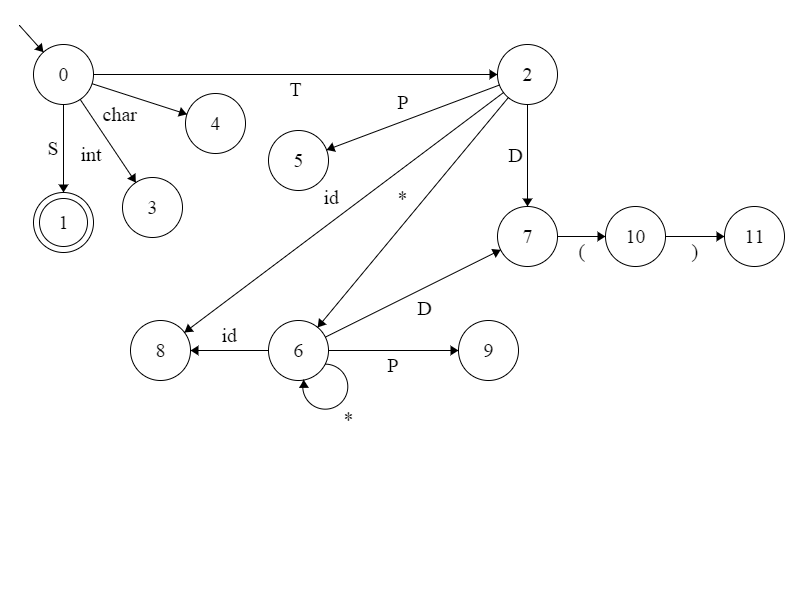
\includegraphics[width=.75\linewidth]{WA04_Exercise01_DFA}
    \label{fig:WA04_Ex01_dfa}
  \end{figure}

  \item Is this grammar SLR(1)? Why or why not?\\\\
  \textit{Answer}:\\\\
  In order to find out if the grammar is SLR(1), we should find out if the
  grammar is ambiguous. We can do so by constructing the parse table. In order to
  construct the parse table, we will need to construct the $Follow$ sets (which also
  requires constructing the $First$ sets), and we will need to assign a numbering to
  the productions of the grammar.\\\\

  First Sets:\\\\
  \begin{tabular}{| r   l |}
  \hline
  $First(S: S \rightarrow T P)$ & $= First(T P)$                      \\
                                & $= First(T) - \{\epsilon\}$         \\
                                & $= \{\texttt{int}, \texttt{char}\}$ \\
  \hline
  \hline
  $First(S)$                    & $= \{\texttt{int}, \texttt{char}\}$ \\
  \hline
  \end{tabular}\\\\

  \begin{tabular}{| r   l |}
  \hline
  $First(T: T \rightarrow \texttt{int})$  & $= First(\texttt{int})$                     \\
                                          & $= \{\texttt{int}\}$                        \\
  \hline
  $First(T: T \rightarrow \texttt{char})$ & $= First(\texttt{char})$                    \\
                                          & $= \{\texttt{char}\}$                       \\
  \hline
  \hline
  $First(T)$                              & $= \{\texttt{int}\} \cup \{\texttt{char}\}$ \\
                                          & $= \{\texttt{int}, \texttt{char}\}$         \\
  \hline
  \end{tabular}\\\\

  \begin{tabular}{| r   l |}
  \hline
  $First(P: P \rightarrow * P)$  & $= First(* P)$                 \\
                                 & $= First(*)$                   \\
                                 & $= \{*\}$                      \\
  \hline
  $First(P: P \rightarrow D$     & $= First(D)$                   \\
                                 & $= \{\texttt{id}\}$            \\
  \hline
  \hline
  $First(P)$                     & $= \{*\} \cup \{\texttt{id}\}$ \\
                                 & $= \{*, \texttt{id}\}$         \\
  \hline
  \end{tabular}\\\\

  \begin{tabular}{| r   l |}
  \hline
  $First(D: D \rightarrow \texttt{id})$   & $= First(\texttt{id})$ \\
                                          & $= \{\texttt{id}\}$    \\
  \hline
  $First(D: D \rightarrow D ( ))$         & $= First(D ( ))$       \\
                                          & $= First(D)$           \\
                                          & $= \texttt{TBD}$       \\
  \hline
  \hline
  $First(D)$                              & $= \{\texttt{id}\}$    \\
  \hline
  \end{tabular}\\\\

  Follow Sets:\\\\
  \begin{tabular}{| r   l |}
  \hline
  $Follow(S: \texttt{Start Symbol})$ & $= \{\$\}$ \\
  \hline
  \hline
  $Follow(S)$                        & $= \{\$\}$ \\
  \hline
  \end{tabular}\\\\

  \begin{tabular}{| r   l |}
  \hline
  $Follow(T: S \rightarrow T P)$ & $= First(P) - \{\epsilon\}$ \\
                                 & $= \{*, \texttt{id}\}$      \\
  \hline
  \hline
  $Follow(T)$                    & $= \{*, \texttt{id}\}$      \\
  \hline
  \end{tabular}\\\\

  \begin{tabular}{| r   l |}
  \hline
  $Follow(P: S \rightarrow T P)$ & $= Follow(S)$    \\
                                 & $= \{\$\}$       \\
  \hline
  $Follow(P: P \rightarrow * P)$ & $= Follow(P)$    \\
                                 & $= \texttt{TBD}$ \\
  \hline
  \hline
  $Follow(P)$                    & $= \{\$\}$       \\
  \hline
  \end{tabular}\\\\

  \begin{tabular}{| r   l |}
  \hline
  $Follow(D: P \rightarrow D)$     & $= Follow(P)$         \\
                                   & $= \{\$\}$            \\
  \hline
  $Follow(D: D \rightarrow D ( ))$ & $= First( ( ) )$      \\
                                   & $= First( ( )$        \\
                                   & $= \{(\}$             \\
  \hline
  \hline
  $Follow(D)$                      & $= \{\$\} \cup \{(\}$ \\
                                   & $= \{(, \$\}$         \\
  \hline
  \end{tabular}\\\\


  Numbered Productions:\\\\
  \begin{tabular}{| c | r   l |}
  \hline
  0 & $Z$ & $\rightarrow \; S$             \\
  \hline
  1 & $S$ & $\rightarrow \; T P$           \\
  \hline
  2 & $T$ & $\rightarrow \; \texttt{int}$  \\
  \hline
  3 & $T$ & $\rightarrow \; \texttt{char}$ \\
  \hline
  4 & $P$ & $\rightarrow \; * P$           \\
  \hline
  5 & $P$ & $\rightarrow \; D$             \\
  \hline
  6 & $D$ & $\rightarrow \; \texttt{id}$   \\
  \hline
  7 & $D$ & $\rightarrow \; D()$           \\
  \hline
  \end{tabular}\\\\

  Action Table:\\\\
  \begin{tabular}{| c || c | c | c | c | c | c | c || c | c | c | c |}
  \hline
        & \multicolumn{7}{| c ||}{Terminals}                                                       & \multicolumn{4}{| c |}{Non-Terminals} \\
  \hline
  State & \texttt{int} & \texttt{char} & \texttt{*} & \texttt{id} & \texttt{(} & \texttt{)} & $\$$ & $S$ & $T$ & $P$ & $D$             \\
  \hline
  \hline
  0     & s3           & s4            &            &             &            &            &      & 1   & 2   &     &                 \\
  \hline
  1     &              &               &            &             &            &            & acc  &     &     &     &                 \\
  \hline
  2     &              &               & s6         & s8          &            &            &      &     &     & 5   & 7               \\
  \hline
  3     &              &               & r2         & r2          &            &            &      &     &     &     &                 \\
  \hline
  4     &              &               & r3         & r3          &            &            &      &     &     &     &                 \\
  \hline
  5     &              &               &            &             &            &            & r1   &     &     &     &                 \\
  \hline
  6     &              &               & s6         & s8          &            &            &      &     &     & 9   & 7               \\
  \hline
  7     &              &               &            &             & s10        &            & r5   &     &     &     &                 \\
  \hline
  8     &              &               &            &             & r6         &            & r6   &     &     &     &                 \\
  \hline
  9     &              &               &            &             &            &            & r4   &     &     &     &                 \\
  \hline
  10    &              &               &            &             &            & s11        &      &     &     &     &                 \\
  \hline
  11    &              &               &            &             & r7         &            & r7   &     &     &     &                 \\
  \hline
  \end{tabular}\\\\

  There were no conflicts in creating the parser table, the grammar is not
  ambiguous, the grammar is an SLR(1) grammar.\\\\

  \newpage
  \item Show the sequence of moves of an SLR(1) parser on the following input. Resolve any
  shift-reduce conflicts in favor of shifting.\\
  \texttt{char } $*$ \texttt{ id()}\\\\
  \textit{Answer}:\\\\
  \textit{Note}: There are no conflicts to resolve.\\\\
  \begin{tabular}{| l | r | l | l |}
  \hline
  \multicolumn{1}{| c |}{Stack}                                         & \multicolumn{1}{| c |}{Input}        & Entry & Action/Production                 \\
  \hline
  \hline
  [(start), 0]                                                          & $\texttt{char } * \texttt{ id()} \$$ & s4    & Shift; Enter State 4              \\
  \hline
  [(start), 0] [\texttt{char}, 4]                                       & $* \texttt{ id()} \$$                & r3    & (3) $T \rightarrow \texttt{char}$ \\
  \hline
  [(start), 0] [T, 2]                                                   & $* \texttt{ id()} \$$                & s6    & Shift; Enter State 6              \\
  \hline
  [(start), 0] [T, 2] [$*$, 6]                                          & $\texttt{id()} \$$                   & s8    & Shift; Enter State 8              \\
  \hline
  [(start), 0] [T, 2] [$*$, 6] [\texttt{id}, 8]                         & $\texttt{()} \$$                     & r6    & (6) $D \rightarrow \texttt{id}$   \\
  \hline
  [(start), 0] [T, 2] [$*$, 6] [D, 7]                                   & $\texttt{()} \$$                     & s10   & Shift; Enter State 10             \\
  \hline
  [(start), 0] [T, 2] [$*$, 6] [D, 7] [\texttt{(}, 10]                  & $\texttt{)} \$$                      & s11   & Shift; Enter State 11             \\
  \hline
  [(start), 0] [T, 2] [$*$, 6] [D, 7] [\texttt{(}, 10] [\texttt{)}, 11] & $\$$                                 & r7    & (7) $D \rightarrow D\texttt{()}$  \\
  \hline
  [(start), 0] [T, 2] [$*$, 6] [D, 7]                                   & $\$$                                 & r5    & (5) $P \rightarrow D$             \\
  \hline
  [(start), 0] [T, 2] [$*$, 6] [P, 9]                                   & $\$$                                 & r4    & (4) $P \rightarrow * P$           \\
  \hline
  [(start), 0] [T, 2] [P, 5]                                            & $\$$                                 & r1    & (1) $S \rightarrow T P$           \\
  \hline   
  [(start), 0] [S, 1]                                                   & $\$$                                 & acc   & \textbf{Successful Parse}         \\
  \hline
  \end{tabular}

\end{enumerate}

\end{document}
